\section{Special effects} \label{sec:specialEffects}
We combined both special effects into one \emph{thing} (it was told form the lectures that this would be okay).


\subsection{Particle System} \label{sec:particleSystem}
Additional to the separate BillboardSGNode described in section~\ref{sec:billboarding} we implemented billboarding in the particle system.
In figure~\ref{fig:particle} you can see our particle system used in the scene.
We decided to set it up as a fire, but any texture would work.


The particle system uses basic quads to render the single fire particles. Each quad has an \emph{starttime} and a \emph{direction}.
Using the starttime, the particle can determine its age and set itself to an appropiate position using
the direction and the origin of the particle system itself.


\begin{figure}[h]
	\centering
	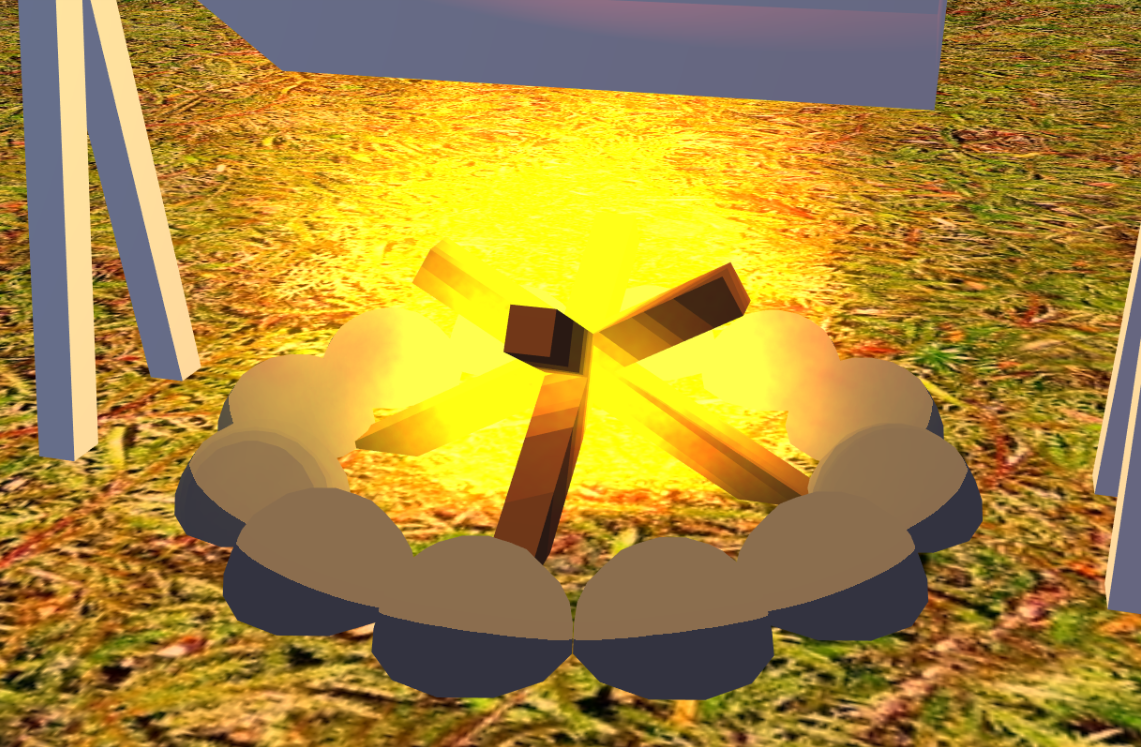
\includegraphics[width=0.5\columnwidth]{figures/particle.png}
	\caption{The fire particle system in action}
	\label{fig:particle}
\end{figure}

The particle system takes 4 arguments:
\begin{itemize}
	\item The texture which it should be applied to the quads (fire in our case)
	\item The frequency of particles, determining how many updates will pass between single spawns of particles
	\item The amount of particles spawned at once
	\item And the maximum amount of particles ever in the system. This is to prevent the infinite creation of particles and therefore crash the program
\end{itemize}

On every update, it is checked whether new particles should be spawned.
If so, the oldest particles are \say{killed} and replaced with new ones with a random direction vector.

We tried to use a particle render method which is based on GL\_POINTS,
which worked for particle systems not close to the camera.
But the size of the point was supplied in pixels, and also we used a approximation $\frac{1}{d}$, where $d$ was the distance
from the camera to the particle, which resulted in wrong approximations when coming close like in our scene.



\subsection{Billboarding} \label{sec:billboarding}
The BillboardSGNode uses  the inverse matrix of the view Matrix to cancel out the rotation.
To leave the object at its world position, the translation parts  of the new matrix are set to zero.